


% Header, overrides base

    % Make sure that the sphinx doc style knows who it inherits from.
    \def\sphinxdocclass{article}

    % Declare the document class
    \documentclass[letterpaper,10pt,english]{/usr/local/lib/python2.7/dist-packages/sphinx/texinputs/sphinxhowto}

    % Imports
    \usepackage[utf8]{inputenc}
    \DeclareUnicodeCharacter{00A0}{\\nobreakspace}
    \usepackage[T1]{fontenc}
    \usepackage{babel}
    \usepackage{times}
    \usepackage{import}
    \usepackage[Bjarne]{/usr/local/lib/python2.7/dist-packages/sphinx/texinputs/fncychap}
    \usepackage{longtable}
    \usepackage{/usr/local/lib/python2.7/dist-packages/sphinx/texinputs/sphinx}
    \usepackage{multirow}

    \usepackage{amsmath}
    \usepackage{amssymb}
    \usepackage{ucs}
    \usepackage{enumerate}

    % Used to make the Input/Output rules follow around the contents.
    \usepackage{needspace}

    % Pygments requirements
    \usepackage{fancyvrb}
    \usepackage{color}
    % ansi colors additions
    \definecolor{darkgreen}{rgb}{.12,.54,.11}
    \definecolor{lightgray}{gray}{.95}
    \definecolor{brown}{rgb}{0.54,0.27,0.07}
    \definecolor{purple}{rgb}{0.5,0.0,0.5}
    \definecolor{darkgray}{gray}{0.25}
    \definecolor{lightred}{rgb}{1.0,0.39,0.28}
    \definecolor{lightgreen}{rgb}{0.48,0.99,0.0}
    \definecolor{lightblue}{rgb}{0.53,0.81,0.92}
    \definecolor{lightpurple}{rgb}{0.87,0.63,0.87}
    \definecolor{lightcyan}{rgb}{0.5,1.0,0.83}

    % Needed to box output/input
    \usepackage{tikz}
        \usetikzlibrary{calc,arrows,shadows}
    \usepackage[framemethod=tikz]{mdframed}

    \usepackage{alltt}

    % Used to load and display graphics
    \usepackage{graphicx}
    \graphicspath{ {figs/} }
    \usepackage[Export]{adjustbox} % To resize

    % used so that images for notebooks which have spaces in the name can still be included
    \usepackage{grffile}


    % For formatting output while also word wrapping.
    \usepackage{listings}
    \lstset{breaklines=true}
    \lstset{basicstyle=\small\ttfamily}
    \def\smaller{\fontsize{9.5pt}{9.5pt}\selectfont}

    %Pygments definitions
    
\makeatletter
\def\PY@reset{\let\PY@it=\relax \let\PY@bf=\relax%
    \let\PY@ul=\relax \let\PY@tc=\relax%
    \let\PY@bc=\relax \let\PY@ff=\relax}
\def\PY@tok#1{\csname PY@tok@#1\endcsname}
\def\PY@toks#1+{\ifx\relax#1\empty\else%
    \PY@tok{#1}\expandafter\PY@toks\fi}
\def\PY@do#1{\PY@bc{\PY@tc{\PY@ul{%
    \PY@it{\PY@bf{\PY@ff{#1}}}}}}}
\def\PY#1#2{\PY@reset\PY@toks#1+\relax+\PY@do{#2}}

\expandafter\def\csname PY@tok@gd\endcsname{\def\PY@tc##1{\textcolor[rgb]{0.63,0.00,0.00}{##1}}}
\expandafter\def\csname PY@tok@gu\endcsname{\let\PY@bf=\textbf\def\PY@tc##1{\textcolor[rgb]{0.50,0.00,0.50}{##1}}}
\expandafter\def\csname PY@tok@gt\endcsname{\def\PY@tc##1{\textcolor[rgb]{0.00,0.27,0.87}{##1}}}
\expandafter\def\csname PY@tok@gs\endcsname{\let\PY@bf=\textbf}
\expandafter\def\csname PY@tok@gr\endcsname{\def\PY@tc##1{\textcolor[rgb]{1.00,0.00,0.00}{##1}}}
\expandafter\def\csname PY@tok@cm\endcsname{\let\PY@it=\textit\def\PY@tc##1{\textcolor[rgb]{0.25,0.50,0.50}{##1}}}
\expandafter\def\csname PY@tok@vg\endcsname{\def\PY@tc##1{\textcolor[rgb]{0.10,0.09,0.49}{##1}}}
\expandafter\def\csname PY@tok@m\endcsname{\def\PY@tc##1{\textcolor[rgb]{0.40,0.40,0.40}{##1}}}
\expandafter\def\csname PY@tok@mh\endcsname{\def\PY@tc##1{\textcolor[rgb]{0.40,0.40,0.40}{##1}}}
\expandafter\def\csname PY@tok@go\endcsname{\def\PY@tc##1{\textcolor[rgb]{0.53,0.53,0.53}{##1}}}
\expandafter\def\csname PY@tok@ge\endcsname{\let\PY@it=\textit}
\expandafter\def\csname PY@tok@vc\endcsname{\def\PY@tc##1{\textcolor[rgb]{0.10,0.09,0.49}{##1}}}
\expandafter\def\csname PY@tok@il\endcsname{\def\PY@tc##1{\textcolor[rgb]{0.40,0.40,0.40}{##1}}}
\expandafter\def\csname PY@tok@cs\endcsname{\let\PY@it=\textit\def\PY@tc##1{\textcolor[rgb]{0.25,0.50,0.50}{##1}}}
\expandafter\def\csname PY@tok@cp\endcsname{\def\PY@tc##1{\textcolor[rgb]{0.74,0.48,0.00}{##1}}}
\expandafter\def\csname PY@tok@gi\endcsname{\def\PY@tc##1{\textcolor[rgb]{0.00,0.63,0.00}{##1}}}
\expandafter\def\csname PY@tok@gh\endcsname{\let\PY@bf=\textbf\def\PY@tc##1{\textcolor[rgb]{0.00,0.00,0.50}{##1}}}
\expandafter\def\csname PY@tok@ni\endcsname{\let\PY@bf=\textbf\def\PY@tc##1{\textcolor[rgb]{0.60,0.60,0.60}{##1}}}
\expandafter\def\csname PY@tok@nl\endcsname{\def\PY@tc##1{\textcolor[rgb]{0.63,0.63,0.00}{##1}}}
\expandafter\def\csname PY@tok@nn\endcsname{\let\PY@bf=\textbf\def\PY@tc##1{\textcolor[rgb]{0.00,0.00,1.00}{##1}}}
\expandafter\def\csname PY@tok@no\endcsname{\def\PY@tc##1{\textcolor[rgb]{0.53,0.00,0.00}{##1}}}
\expandafter\def\csname PY@tok@na\endcsname{\def\PY@tc##1{\textcolor[rgb]{0.49,0.56,0.16}{##1}}}
\expandafter\def\csname PY@tok@nb\endcsname{\def\PY@tc##1{\textcolor[rgb]{0.00,0.50,0.00}{##1}}}
\expandafter\def\csname PY@tok@nc\endcsname{\let\PY@bf=\textbf\def\PY@tc##1{\textcolor[rgb]{0.00,0.00,1.00}{##1}}}
\expandafter\def\csname PY@tok@nd\endcsname{\def\PY@tc##1{\textcolor[rgb]{0.67,0.13,1.00}{##1}}}
\expandafter\def\csname PY@tok@ne\endcsname{\let\PY@bf=\textbf\def\PY@tc##1{\textcolor[rgb]{0.82,0.25,0.23}{##1}}}
\expandafter\def\csname PY@tok@nf\endcsname{\def\PY@tc##1{\textcolor[rgb]{0.00,0.00,1.00}{##1}}}
\expandafter\def\csname PY@tok@si\endcsname{\let\PY@bf=\textbf\def\PY@tc##1{\textcolor[rgb]{0.73,0.40,0.53}{##1}}}
\expandafter\def\csname PY@tok@s2\endcsname{\def\PY@tc##1{\textcolor[rgb]{0.73,0.13,0.13}{##1}}}
\expandafter\def\csname PY@tok@vi\endcsname{\def\PY@tc##1{\textcolor[rgb]{0.10,0.09,0.49}{##1}}}
\expandafter\def\csname PY@tok@nt\endcsname{\let\PY@bf=\textbf\def\PY@tc##1{\textcolor[rgb]{0.00,0.50,0.00}{##1}}}
\expandafter\def\csname PY@tok@nv\endcsname{\def\PY@tc##1{\textcolor[rgb]{0.10,0.09,0.49}{##1}}}
\expandafter\def\csname PY@tok@s1\endcsname{\def\PY@tc##1{\textcolor[rgb]{0.73,0.13,0.13}{##1}}}
\expandafter\def\csname PY@tok@kd\endcsname{\let\PY@bf=\textbf\def\PY@tc##1{\textcolor[rgb]{0.00,0.50,0.00}{##1}}}
\expandafter\def\csname PY@tok@sh\endcsname{\def\PY@tc##1{\textcolor[rgb]{0.73,0.13,0.13}{##1}}}
\expandafter\def\csname PY@tok@sc\endcsname{\def\PY@tc##1{\textcolor[rgb]{0.73,0.13,0.13}{##1}}}
\expandafter\def\csname PY@tok@sx\endcsname{\def\PY@tc##1{\textcolor[rgb]{0.00,0.50,0.00}{##1}}}
\expandafter\def\csname PY@tok@bp\endcsname{\def\PY@tc##1{\textcolor[rgb]{0.00,0.50,0.00}{##1}}}
\expandafter\def\csname PY@tok@c1\endcsname{\let\PY@it=\textit\def\PY@tc##1{\textcolor[rgb]{0.25,0.50,0.50}{##1}}}
\expandafter\def\csname PY@tok@kc\endcsname{\let\PY@bf=\textbf\def\PY@tc##1{\textcolor[rgb]{0.00,0.50,0.00}{##1}}}
\expandafter\def\csname PY@tok@c\endcsname{\let\PY@it=\textit\def\PY@tc##1{\textcolor[rgb]{0.25,0.50,0.50}{##1}}}
\expandafter\def\csname PY@tok@mf\endcsname{\def\PY@tc##1{\textcolor[rgb]{0.40,0.40,0.40}{##1}}}
\expandafter\def\csname PY@tok@err\endcsname{\def\PY@bc##1{\setlength{\fboxsep}{0pt}\fcolorbox[rgb]{1.00,0.00,0.00}{1,1,1}{\strut ##1}}}
\expandafter\def\csname PY@tok@mb\endcsname{\def\PY@tc##1{\textcolor[rgb]{0.40,0.40,0.40}{##1}}}
\expandafter\def\csname PY@tok@ss\endcsname{\def\PY@tc##1{\textcolor[rgb]{0.10,0.09,0.49}{##1}}}
\expandafter\def\csname PY@tok@sr\endcsname{\def\PY@tc##1{\textcolor[rgb]{0.73,0.40,0.53}{##1}}}
\expandafter\def\csname PY@tok@mo\endcsname{\def\PY@tc##1{\textcolor[rgb]{0.40,0.40,0.40}{##1}}}
\expandafter\def\csname PY@tok@kn\endcsname{\let\PY@bf=\textbf\def\PY@tc##1{\textcolor[rgb]{0.00,0.50,0.00}{##1}}}
\expandafter\def\csname PY@tok@mi\endcsname{\def\PY@tc##1{\textcolor[rgb]{0.40,0.40,0.40}{##1}}}
\expandafter\def\csname PY@tok@gp\endcsname{\let\PY@bf=\textbf\def\PY@tc##1{\textcolor[rgb]{0.00,0.00,0.50}{##1}}}
\expandafter\def\csname PY@tok@o\endcsname{\def\PY@tc##1{\textcolor[rgb]{0.40,0.40,0.40}{##1}}}
\expandafter\def\csname PY@tok@kr\endcsname{\let\PY@bf=\textbf\def\PY@tc##1{\textcolor[rgb]{0.00,0.50,0.00}{##1}}}
\expandafter\def\csname PY@tok@s\endcsname{\def\PY@tc##1{\textcolor[rgb]{0.73,0.13,0.13}{##1}}}
\expandafter\def\csname PY@tok@kp\endcsname{\def\PY@tc##1{\textcolor[rgb]{0.00,0.50,0.00}{##1}}}
\expandafter\def\csname PY@tok@w\endcsname{\def\PY@tc##1{\textcolor[rgb]{0.73,0.73,0.73}{##1}}}
\expandafter\def\csname PY@tok@kt\endcsname{\def\PY@tc##1{\textcolor[rgb]{0.69,0.00,0.25}{##1}}}
\expandafter\def\csname PY@tok@ow\endcsname{\let\PY@bf=\textbf\def\PY@tc##1{\textcolor[rgb]{0.67,0.13,1.00}{##1}}}
\expandafter\def\csname PY@tok@sb\endcsname{\def\PY@tc##1{\textcolor[rgb]{0.73,0.13,0.13}{##1}}}
\expandafter\def\csname PY@tok@k\endcsname{\let\PY@bf=\textbf\def\PY@tc##1{\textcolor[rgb]{0.00,0.50,0.00}{##1}}}
\expandafter\def\csname PY@tok@se\endcsname{\let\PY@bf=\textbf\def\PY@tc##1{\textcolor[rgb]{0.73,0.40,0.13}{##1}}}
\expandafter\def\csname PY@tok@sd\endcsname{\let\PY@it=\textit\def\PY@tc##1{\textcolor[rgb]{0.73,0.13,0.13}{##1}}}

\def\PYZbs{\char`\\}
\def\PYZus{\char`\_}
\def\PYZob{\char`\{}
\def\PYZcb{\char`\}}
\def\PYZca{\char`\^}
\def\PYZam{\char`\&}
\def\PYZlt{\char`\<}
\def\PYZgt{\char`\>}
\def\PYZsh{\char`\#}
\def\PYZpc{\char`\%}
\def\PYZdl{\char`\$}
\def\PYZhy{\char`\-}
\def\PYZsq{\char`\'}
\def\PYZdq{\char`\"}
\def\PYZti{\char`\~}
% for compatibility with earlier versions
\def\PYZat{@}
\def\PYZlb{[}
\def\PYZrb{]}
\makeatother


    %Set pygments styles if needed...
    
        \definecolor{nbframe-border}{rgb}{0.867,0.867,0.867}
        \definecolor{nbframe-bg}{rgb}{0.969,0.969,0.969}
        \definecolor{nbframe-in-prompt}{rgb}{0.0,0.0,0.502}
        \definecolor{nbframe-out-prompt}{rgb}{0.545,0.0,0.0}

        \newenvironment{ColorVerbatim}
        {\begin{mdframed}[%
            roundcorner=1.0pt, %
            backgroundcolor=nbframe-bg, %
            userdefinedwidth=1\linewidth, %
            leftmargin=0.1\linewidth, %
            innerleftmargin=0pt, %
            innerrightmargin=0pt, %
            linecolor=nbframe-border, %
            linewidth=1pt, %
            usetwoside=false, %
            everyline=true, %
            innerlinewidth=3pt, %
            innerlinecolor=nbframe-bg, %
            middlelinewidth=1pt, %
            middlelinecolor=nbframe-bg, %
            outerlinewidth=0.5pt, %
            outerlinecolor=nbframe-border, %
            needspace=0pt
        ]}
        {\end{mdframed}}
        
        \newenvironment{InvisibleVerbatim}
        {\begin{mdframed}[leftmargin=0.1\linewidth,innerleftmargin=3pt,innerrightmargin=3pt, userdefinedwidth=1\linewidth, linewidth=0pt, linecolor=white, usetwoside=false]}
        {\end{mdframed}}

        \renewenvironment{Verbatim}[1][\unskip]
        {\begin{alltt}\smaller}
        {\end{alltt}}
    

    % Help prevent overflowing lines due to urls and other hard-to-break 
    % entities.  This doesn't catch everything...
    \sloppy

    % Document level variables
    \title{WavesPset10}
    \date{November 23, 2014}
    \release{}
    \author{Unknown Author}
    \renewcommand{\releasename}{}

    % TODO: Add option for the user to specify a logo for his/her export.
    \newcommand{\sphinxlogo}{}

    % Make the index page of the document.
    \makeindex

    % Import sphinx document type specifics.
     


% Body

    % Start of the document
    \begin{document}

        
            \maketitle
        

        


        
        \section{Problem Set 10, by Chris Silvia}\subsubsection{Problem 2.5}For an Einstein solid with each of the following values of \(N\) and
\(q\), list all of the possible microstates.The number of einstein microstates is the same as the number of ways to
put \(q\) balls in \(N\) slots.

0 0 0 \textbar{} \textbar{} 0 0 \textbar{}

There are \(N + q - 1\) possible places to put things in general, and
choices of where the slots are (\(q\) of them) uniquely determine the
formula.

\[
\Omega(N,q) = {{q + N -1} \choose q}
\]

    % Make sure that atleast 4 lines are below the HR
    \needspace{4\baselineskip}

    
        \vspace{6pt}
        \makebox[0.1\linewidth]{\smaller\hfill\tt\color{nbframe-in-prompt}In\hspace{4pt}{[}28{]}:\hspace{4pt}}\\*
        \vspace{-2.65\baselineskip}
        \begin{ColorVerbatim}
            \vspace{-0.7\baselineskip}
            \begin{Verbatim}[commandchars=\\\{\}]
\PY{k+kn}{import} \PY{n+nn}{numpy} \PY{k+kn}{as} \PY{n+nn}{np}

\PY{k}{def} \PY{n+nf}{fact}\PY{p}{(}\PY{n}{n}\PY{p}{)}\PY{p}{:}
    \PY{n}{i} \PY{o}{=} \PY{l+m+mi}{1}
    \PY{k}{for} \PY{n}{j} \PY{o+ow}{in} \PY{n+nb}{range}\PY{p}{(}\PY{l+m+mi}{1}\PY{p}{,}\PY{n}{n}\PY{o}{+}\PY{l+m+mi}{1}\PY{p}{)}\PY{p}{:}
        \PY{n}{i} \PY{o}{*}\PY{o}{=} \PY{n}{j}
    \PY{k}{return} \PY{n}{i}

\PY{k}{def} \PY{n+nf}{choose}\PY{p}{(}\PY{n}{n}\PY{p}{,}\PY{n}{k}\PY{p}{)}\PY{p}{:}
    \PY{l+s+sd}{\PYZdq{}\PYZdq{}\PYZdq{}Computes n choose k\PYZdq{}\PYZdq{}\PYZdq{}}
    \PY{k}{return} \PY{n}{fact}\PY{p}{(}\PY{n}{n}\PY{p}{)}\PY{o}{/}\PY{p}{(}\PY{n}{fact}\PY{p}{(}\PY{n}{n}\PY{o}{\PYZhy{}}\PY{n}{k}\PY{p}{)} \PY{o}{*} \PY{n}{fact}\PY{p}{(}\PY{n}{k}\PY{p}{)}\PY{p}{)}

\PY{k}{def} \PY{n+nf}{einstein\PYZus{}solid}\PY{p}{(}\PY{n}{N}\PY{p}{,}\PY{n}{q}\PY{p}{)}\PY{p}{:}
    \PY{l+s+sd}{\PYZdq{}\PYZdq{}\PYZdq{}Number of states for an einstein solid }
\PY{l+s+sd}{    with N oscillators and q units of energy. }
\PY{l+s+sd}{    Returns an integer\PYZdq{}\PYZdq{}\PYZdq{}}
    \PY{k}{return} \PY{n}{choose}\PY{p}{(}\PY{n}{q} \PY{o}{+} \PY{n}{N} \PY{o}{\PYZhy{}} \PY{l+m+mi}{1}\PY{p}{,}\PY{n}{q}\PY{p}{)}

\PY{k}{def} \PY{n+nf}{einstein\PYZus{}solid\PYZus{}microstates}\PY{p}{(}\PY{n}{N}\PY{p}{,}\PY{n}{q}\PY{p}{)}\PY{p}{:}
    \PY{l+s+sd}{\PYZdq{}\PYZdq{}\PYZdq{}Lists, explicitly, the microstates for an}
\PY{l+s+sd}{    einstein solid of N oscillators with q units of}
\PY{l+s+sd}{    energy.  THIS IS RECURSIVE, don\PYZsq{}t do big things\PYZdq{}\PYZdq{}\PYZdq{}}
    \PY{n}{states} \PY{o}{=} \PY{p}{[}\PY{p}{]}
    \PY{k}{if} \PY{n}{N} \PY{o}{==} \PY{l+m+mi}{1}\PY{p}{:}
        \PY{k}{return} \PY{p}{[}\PY{p}{[}\PY{n}{q}\PY{p}{]}\PY{p}{]}
    \PY{k}{elif} \PY{n}{q} \PY{o}{==} \PY{l+m+mi}{0}\PY{p}{:}
        \PY{k}{return} \PY{p}{[}\PY{p}{[}\PY{l+m+mi}{0} \PY{k}{for} \PY{n}{i} \PY{o+ow}{in} \PY{n+nb}{range}\PY{p}{(}\PY{l+m+mi}{0}\PY{p}{,}\PY{n}{N}\PY{p}{)}\PY{p}{]}\PY{p}{]}
    \PY{k}{elif} \PY{n}{q} \PY{o}{==} \PY{l+m+mi}{1}\PY{p}{:}
        \PY{k}{for} \PY{n}{i} \PY{o+ow}{in} \PY{n+nb}{range}\PY{p}{(}\PY{l+m+mi}{0}\PY{p}{,}\PY{n}{N}\PY{p}{)}\PY{p}{:}
            \PY{n}{states} \PY{o}{+}\PY{o}{=} \PY{p}{[}\PY{p}{[} \PY{l+m+mi}{1} \PY{k}{if} \PY{n}{n} \PY{o}{==} \PY{n}{i} \PY{k}{else} \PY{l+m+mi}{0} \PY{k}{for} \PY{n}{n} \PY{o+ow}{in} \PY{n+nb}{range}\PY{p}{(}\PY{l+m+mi}{0}\PY{p}{,}\PY{n}{N}\PY{p}{)}\PY{p}{]}\PY{p}{]}
        \PY{k}{return} \PY{n}{states}
    \PY{k}{else}\PY{p}{:}
        \PY{k}{for} \PY{n}{i} \PY{o+ow}{in} \PY{n+nb}{range}\PY{p}{(}\PY{l+m+mi}{0}\PY{p}{,}\PY{n}{q}\PY{o}{+}\PY{l+m+mi}{1}\PY{p}{)}\PY{p}{:}
            \PY{n}{states} \PY{o}{+}\PY{o}{=} \PY{p}{[}\PY{p}{[}\PY{n}{i}\PY{p}{]}\PY{o}{+}\PY{n}{xtail} \PY{k}{for} \PY{n}{xtail} \PY{o+ow}{in} \PY{n}{einstein\PYZus{}solid\PYZus{}microstates}\PY{p}{(}\PY{n}{N}\PY{o}{\PYZhy{}}\PY{l+m+mi}{1}\PY{p}{,}\PY{n}{q}\PY{o}{\PYZhy{}}\PY{n}{i}\PY{p}{)}\PY{p}{]}
        \PY{k}{return} \PY{n}{states}
        

\PY{n}{data} \PY{o}{=} \PY{p}{[}\PY{p}{(}\PY{l+s}{\PYZdq{}}\PY{l+s}{a}\PY{l+s}{\PYZdq{}}\PY{p}{,}\PY{l+m+mi}{3}\PY{p}{,}\PY{l+m+mi}{4}\PY{p}{)}\PY{p}{,}\PY{p}{(}\PY{l+s}{\PYZdq{}}\PY{l+s}{b}\PY{l+s}{\PYZdq{}}\PY{p}{,}\PY{l+m+mi}{3}\PY{p}{,}\PY{l+m+mi}{5}\PY{p}{)}\PY{p}{,}\PY{p}{(}\PY{l+s}{\PYZdq{}}\PY{l+s}{c}\PY{l+s}{\PYZdq{}}\PY{p}{,}\PY{l+m+mi}{3}\PY{p}{,}\PY{l+m+mi}{6}\PY{p}{)}\PY{p}{,}\PY{p}{(}\PY{l+s}{\PYZdq{}}\PY{l+s}{d}\PY{l+s}{\PYZdq{}}\PY{p}{,}\PY{l+m+mi}{4}\PY{p}{,}\PY{l+m+mi}{2}\PY{p}{)}\PY{p}{,}\PY{p}{(}\PY{l+s}{\PYZdq{}}\PY{l+s}{e}\PY{l+s}{\PYZdq{}}\PY{p}{,}\PY{l+m+mi}{4}\PY{p}{,}\PY{l+m+mi}{3}\PY{p}{)}\PY{p}{]}

\PY{k}{for} \PY{n}{number}\PY{p}{,}\PY{n}{N}\PY{p}{,}\PY{n}{q} \PY{o+ow}{in} \PY{n}{data}\PY{p}{:}
    \PY{k}{print} \PY{l+s}{\PYZdq{}}\PY{l+s}{\PYZob{}0\PYZcb{}: N=\PYZob{}1\PYZcb{} q=\PYZob{}2\PYZcb{} n\PYZus{}microstates=\PYZob{}3\PYZcb{}}\PY{l+s+se}{\PYZbs{}n}\PY{l+s}{The actual microstates:}\PY{l+s+se}{\PYZbs{}n}\PY{l+s}{\PYZob{}4\PYZcb{}}\PY{l+s}{\PYZdq{}}\PY{o}{.}\PY{n}{format}\PY{p}{(}
    \PY{n}{number}\PY{p}{,}\PY{n}{N}\PY{p}{,}\PY{n}{q}\PY{p}{,}\PY{n}{einstein\PYZus{}solid}\PY{p}{(}\PY{n}{N}\PY{p}{,}\PY{n}{q}\PY{p}{)}\PY{p}{,}\PY{n}{einstein\PYZus{}solid\PYZus{}microstates}\PY{p}{(}\PY{n}{N}\PY{p}{,}\PY{n}{q}\PY{p}{)}\PY{p}{)}
\end{Verbatim}

            
                \vspace{-0.2\baselineskip}
            
        \end{ColorVerbatim}
    

    

        % If the first block is an image, minipage the image.  Else
        % request a certain amount of space for the input text.
        \needspace{4\baselineskip}
        
        

            % Add document contents.
            
                \begin{InvisibleVerbatim}
                \vspace{-0.5\baselineskip}
\begin{alltt}a: N=3 q=4 n\_microstates=15
The actual microstates:
[[0, 0, 4], [0, 1, 3], [0, 2, 2], [0, 3, 1], [0, 4, 0], [1, 0, 3], [1,
1, 2], [1, 2, 1], [1, 3, 0], [2, 0, 2], [2, 1, 1], [2, 2, 0], [3, 1,
0], [3, 0, 1], [4, 0, 0]]
b: N=3 q=5 n\_microstates=21
The actual microstates:
[[0, 0, 5], [0, 1, 4], [0, 2, 3], [0, 3, 2], [0, 4, 1], [0, 5, 0], [1,
0, 4], [1, 1, 3], [1, 2, 2], [1, 3, 1], [1, 4, 0], [2, 0, 3], [2, 1,
2], [2, 2, 1], [2, 3, 0], [3, 0, 2], [3, 1, 1], [3, 2, 0], [4, 1, 0],
[4, 0, 1], [5, 0, 0]]
c: N=3 q=6 n\_microstates=28
The actual microstates:
[[0, 0, 6], [0, 1, 5], [0, 2, 4], [0, 3, 3], [0, 4, 2], [0, 5, 1], [0,
6, 0], [1, 0, 5], [1, 1, 4], [1, 2, 3], [1, 3, 2], [1, 4, 1], [1, 5,
0], [2, 0, 4], [2, 1, 3], [2, 2, 2], [2, 3, 1], [2, 4, 0], [3, 0, 3],
[3, 1, 2], [3, 2, 1], [3, 3, 0], [4, 0, 2], [4, 1, 1], [4, 2, 0], [5,
1, 0], [5, 0, 1], [6, 0, 0]]
d: N=4 q=2 n\_microstates=10
The actual microstates:
[[0, 0, 0, 2], [0, 0, 1, 1], [0, 0, 2, 0], [0, 1, 1, 0], [0, 1, 0, 1],
[0, 2, 0, 0], [1, 1, 0, 0], [1, 0, 1, 0], [1, 0, 0, 1], [2, 0, 0, 0]]
e: N=4 q=3 n\_microstates=20
The actual microstates:
[[0, 0, 0, 3], [0, 0, 1, 2], [0, 0, 2, 1], [0, 0, 3, 0], [0, 1, 0, 2],
[0, 1, 1, 1], [0, 1, 2, 0], [0, 2, 1, 0], [0, 2, 0, 1], [0, 3, 0, 0],
[1, 0, 0, 2], [1, 0, 1, 1], [1, 0, 2, 0], [1, 1, 1, 0], [1, 1, 0, 1],
[1, 2, 0, 0], [2, 1, 0, 0], [2, 0, 1, 0], [2, 0, 0, 1], [3, 0, 0, 0]]
\end{alltt}

            \end{InvisibleVerbatim}
            
        
    
\begin{enumerate}
\def\labelenumi{\alph{enumi})}
\setcounter{enumi}{5}
\itemsep1pt\parskip0pt\parsep0pt
\item
  When \(N = 1\), there is exactly one way of putting all the energy
  into that one box.
\end{enumerate}\begin{enumerate}
\def\labelenumi{\alph{enumi})}
\setcounter{enumi}{6}
\itemsep1pt\parskip0pt\parsep0pt
\item
  When \(q = 1\), there are \(N \choose q\) ways of putting the one
  quantum of energy into each of the \(N\) oscillators.
\end{enumerate}\subsubsection{Problem 2.6}Want: multiplicity of an einstein solid with \(N = 30\) and \(q = 30\).

    % Make sure that atleast 4 lines are below the HR
    \needspace{4\baselineskip}

    
        \vspace{6pt}
        \makebox[0.1\linewidth]{\smaller\hfill\tt\color{nbframe-in-prompt}In\hspace{4pt}{[}8{]}:\hspace{4pt}}\\*
        \vspace{-2.65\baselineskip}
        \begin{ColorVerbatim}
            \vspace{-0.7\baselineskip}
            \begin{Verbatim}[commandchars=\\\{\}]
\PY{k}{print} \PY{l+s}{\PYZdq{}}\PY{l+s}{There are \PYZob{}0\PYZcb{} states for an einstein solid with 30 oscillators and 30 units of energy}\PY{l+s}{\PYZdq{}}\PY{o}{.}\PY{n}{format}\PY{p}{(}\PY{n}{einstein\PYZus{}solid}\PY{p}{(}\PY{l+m+mi}{30}\PY{p}{,}\PY{l+m+mi}{30}\PY{p}{)}\PY{p}{)}
\end{Verbatim}

            
                \vspace{-0.2\baselineskip}
            
        \end{ColorVerbatim}
    

    

        % If the first block is an image, minipage the image.  Else
        % request a certain amount of space for the input text.
        \needspace{4\baselineskip}
        
        

            % Add document contents.
            
                \begin{InvisibleVerbatim}
                \vspace{-0.5\baselineskip}
\begin{alltt}There are 59132290782430712 states for an einstein solid with 30
oscillators and 30 units of energy
\end{alltt}

            \end{InvisibleVerbatim}
            
        
    
\subsubsection{Problem 2.8}Consider a system of two einstein solids \(A\) and \(B\), each
containing 10 oscillators, with at total of 20 units of energy. The
solids are weakly coupled and total energy is fixed.

Macrostates can only be distinguished by how much total energy is in
\(A\) and not \(B\), or vice versa.

    % Make sure that atleast 4 lines are below the HR
    \needspace{4\baselineskip}

    
        \vspace{6pt}
        \makebox[0.1\linewidth]{\smaller\hfill\tt\color{nbframe-in-prompt}In\hspace{4pt}{[}57{]}:\hspace{4pt}}\\*
        \vspace{-2.65\baselineskip}
        \begin{ColorVerbatim}
            \vspace{-0.7\baselineskip}
            \begin{Verbatim}[commandchars=\\\{\}]
\PY{n}{q} \PY{o}{=} \PY{l+m+mi}{20}

\PY{n}{microstates} \PY{o}{=} \PY{p}{[} \PY{n}{einstein\PYZus{}solid}\PY{p}{(}\PY{l+m+mi}{10}\PY{p}{,}\PY{n}{qa}\PY{p}{)}\PY{o}{*}\PY{n}{einstein\PYZus{}solid}\PY{p}{(}\PY{l+m+mi}{10}\PY{p}{,}\PY{n}{q}\PY{o}{\PYZhy{}}\PY{n}{qa}\PY{p}{)} \PY{k}{for} \PY{n}{qa} \PY{o+ow}{in} \PY{n+nb}{range}\PY{p}{(}\PY{l+m+mi}{0}\PY{p}{,}\PY{l+m+mi}{20}\PY{o}{+}\PY{l+m+mi}{1}\PY{p}{)}\PY{p}{]}
\PY{n}{n\PYZus{}microstates} \PY{o}{=} \PY{n+nb}{sum}\PY{p}{(}\PY{n}{microstates}\PY{p}{)}
\PY{n}{normalized\PYZus{}microstates} \PY{o}{=} \PY{p}{[}\PY{n+nb}{float}\PY{p}{(}\PY{n}{omega}\PY{p}{)}\PY{o}{/}\PY{n+nb}{float}\PY{p}{(}\PY{n}{n\PYZus{}microstates}\PY{p}{)} \PY{k}{for} \PY{n}{omega} \PY{o+ow}{in} \PY{n}{microstates}\PY{p}{]}

\PY{k}{print} \PY{l+s}{\PYZdq{}}\PY{l+s}{a) There are \PYZob{}0\PYZcb{} macrostates}\PY{l+s}{\PYZdq{}}\PY{o}{.}\PY{n}{format}\PY{p}{(}\PY{n+nb}{len}\PY{p}{(}\PY{n}{microstates}\PY{p}{)}\PY{p}{)}
\PY{k}{print} \PY{l+s}{\PYZdq{}}\PY{l+s}{b) There are \PYZob{}0\PYZcb{} microstates}\PY{l+s}{\PYZdq{}}\PY{o}{.}\PY{n}{format}\PY{p}{(}\PY{n+nb}{sum}\PY{p}{(}\PY{n}{microstates}\PY{p}{)}\PY{p}{)}
\PY{k}{print} \PY{l+s}{\PYZdq{}}\PY{l+s}{c) The probability of all the energy in A is \PYZob{}0\PYZcb{}}\PY{l+s}{\PYZdq{}}\PY{o}{.}\PY{n}{format}\PY{p}{(}\PY{n}{normalized\PYZus{}microstates}\PY{p}{[}\PY{l+m+mi}{20}\PY{p}{]}\PY{p}{)}
\PY{k}{print} \PY{l+s}{\PYZdq{}}\PY{l+s}{d) The probability of finding half the energy in A is \PYZob{}0\PYZcb{}}\PY{l+s}{\PYZdq{}}\PY{o}{.}\PY{n}{format}\PY{p}{(}\PY{n}{normalized\PYZus{}microstates}\PY{p}{[}\PY{l+m+mi}{10}\PY{p}{]}\PY{p}{)}
\end{Verbatim}

            
                \vspace{-0.2\baselineskip}
            
        \end{ColorVerbatim}
    

    

        % If the first block is an image, minipage the image.  Else
        % request a certain amount of space for the input text.
        \needspace{4\baselineskip}
        
        

            % Add document contents.
            
                \begin{InvisibleVerbatim}
                \vspace{-0.5\baselineskip}
\begin{alltt}a) There are 21 macrostates
b) There are 68923264410 microstates
c) The probability of all the energy in A is 0.00014530659692
d) The probability of finding half the energy in A is 0.123814432718
\end{alltt}

            \end{InvisibleVerbatim}
            
        
    
\begin{enumerate}
\def\labelenumi{\alph{enumi})}
\setcounter{enumi}{4}
\itemsep1pt\parskip0pt\parsep0pt
\item
  The system would exhibit irreversible behavior if the system starts
  out initially in a very unlikely state.
\end{enumerate}\subsubsection{Problem 2.10}This graph is interactions between an einstein solid \(A\) with
\(N_A = 200\) oscillators and an einstein solid \(B\) with \(N_B = 100\)
oscillators. There are 100 units of energy in total.

    % Make sure that atleast 4 lines are below the HR
    \needspace{4\baselineskip}

    
        \vspace{6pt}
        \makebox[0.1\linewidth]{\smaller\hfill\tt\color{nbframe-in-prompt}In\hspace{4pt}{[}55{]}:\hspace{4pt}}\\*
        \vspace{-2.65\baselineskip}
        \begin{ColorVerbatim}
            \vspace{-0.7\baselineskip}
            \begin{Verbatim}[commandchars=\\\{\}]
\PY{o}{\PYZpc{}}\PY{k}{matplotlib} \PY{n}{inline}
\PY{k+kn}{import} \PY{n+nn}{numpy} \PY{k+kn}{as} \PY{n+nn}{np}

\PY{k+kn}{import} \PY{n+nn}{matplotlib.pyplot} \PY{k+kn}{as} \PY{n+nn}{plt}

\PY{n}{NA}\PY{p}{,}\PY{n}{NB} \PY{o}{=} \PY{l+m+mi}{200}\PY{p}{,}\PY{l+m+mi}{100}
\PY{n}{q} \PY{o}{=} \PY{l+m+mi}{100}

\PY{n}{qadistribution} \PY{o}{=} \PY{p}{[} \PY{n}{einstein\PYZus{}solid}\PY{p}{(}\PY{n}{NA}\PY{p}{,}\PY{n}{qa}\PY{p}{)}\PY{o}{*}\PY{n}{einstein\PYZus{}solid}\PY{p}{(}\PY{n}{NB}\PY{p}{,}\PY{n}{q}\PY{o}{\PYZhy{}}\PY{n}{qa}\PY{p}{)} \PY{k}{for} \PY{n}{qa} \PY{o+ow}{in} \PY{n+nb}{range}\PY{p}{(}\PY{l+m+mi}{0}\PY{p}{,}\PY{l+m+mi}{100}\PY{o}{+}\PY{l+m+mi}{1}\PY{p}{)}\PY{p}{]}
\PY{n}{n\PYZus{}microstates} \PY{o}{=} \PY{n+nb}{sum}\PY{p}{(}\PY{n}{qadistribution}\PY{p}{)}
\PY{n}{normalized\PYZus{}qadistribution} \PY{o}{=} \PY{p}{[}\PY{n+nb}{float}\PY{p}{(}\PY{n}{omega}\PY{p}{)} \PY{o}{/} \PY{n+nb}{float}\PY{p}{(}\PY{n}{n\PYZus{}microstates}\PY{p}{)} \PY{k}{for} \PY{n}{omega} \PY{o+ow}{in} \PY{n}{qadistribution}\PY{p}{]}

\PY{k}{print} \PY{l+s}{\PYZdq{}}\PY{l+s}{The most probable state where qa = \PYZob{}1\PYZcb{} has a probability of \PYZob{}0\PYZcb{}}\PY{l+s}{\PYZdq{}}\PY{o}{.}\PY{n}{format}\PY{p}{(}
        \PY{n+nb}{max}\PY{p}{(}\PY{n}{normalized\PYZus{}qadistribution}\PY{p}{)}\PY{p}{,}\PY{n}{np}\PY{o}{.}\PY{n}{argmax}\PY{p}{(}\PY{n}{normalized\PYZus{}qadistribution}\PY{p}{)}\PY{p}{)}
\PY{k}{print} \PY{l+s}{\PYZdq{}}\PY{l+s}{The least probable state where qa = \PYZob{}1\PYZcb{} has a probability of \PYZob{}0\PYZcb{}}\PY{l+s}{\PYZdq{}}\PY{o}{.}\PY{n}{format}\PY{p}{(}
        \PY{n+nb}{min}\PY{p}{(}\PY{n}{normalized\PYZus{}qadistribution}\PY{p}{)}\PY{p}{,}\PY{n}{np}\PY{o}{.}\PY{n}{argmin}\PY{p}{(}\PY{n}{normalized\PYZus{}qadistribution}\PY{p}{)}\PY{p}{)}
\PY{n}{plt}\PY{o}{.}\PY{n}{title}\PY{p}{(}\PY{l+s}{\PYZdq{}}\PY{l+s}{Energy Probability Distribution}\PY{l+s}{\PYZdq{}}\PY{p}{)}
\PY{n}{plt}\PY{o}{.}\PY{n}{xlabel}\PY{p}{(}\PY{l+s}{\PYZdq{}}\PY{l+s}{q\PYZus{}a}\PY{l+s}{\PYZdq{}}\PY{p}{)}
\PY{n}{plt}\PY{o}{.}\PY{n}{ylabel}\PY{p}{(}\PY{l+s}{\PYZdq{}}\PY{l+s}{probability}\PY{l+s}{\PYZdq{}}\PY{p}{)}
\PY{n}{plt}\PY{o}{.}\PY{n}{plot}\PY{p}{(}\PY{n+nb}{range}\PY{p}{(}\PY{l+m+mi}{0}\PY{p}{,}\PY{l+m+mi}{101}\PY{p}{)}\PY{p}{,}\PY{n}{normalized\PYZus{}qadistribution}\PY{p}{)}
\end{Verbatim}

            
                \vspace{-0.2\baselineskip}
            
        \end{ColorVerbatim}
    

    

        % If the first block is an image, minipage the image.  Else
        % request a certain amount of space for the input text.
        \needspace{4\baselineskip}
        
        

            % Add document contents.
            
                \begin{InvisibleVerbatim}
                \vspace{-0.5\baselineskip}
\begin{alltt}The most probable state where qa = 67 has a probability of
0.073151397822
The least probable state where qa = 0 has a probability of
2.69266665552e-38
\end{alltt}

            \end{InvisibleVerbatim}
            
                \makebox[0.1\linewidth]{\smaller\hfill\tt\color{nbframe-out-prompt}Out\hspace{4pt}{[}55{]}:\hspace{4pt}}\\*
                \vspace{-2.55\baselineskip}\begin{InvisibleVerbatim}
                \vspace{-0.5\baselineskip}
\begin{alltt}[<matplotlib.lines.Line2D at 0xb012ec0c>]\end{alltt}

            \end{InvisibleVerbatim}
            
                \begin{InvisibleVerbatim}
                \vspace{-0.5\baselineskip}
    \begin{center}
    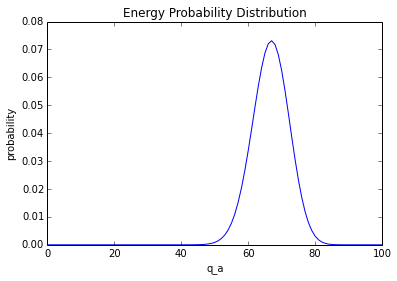
\includegraphics[max size={\textwidth}{\textheight}]{WavesPset10_files/WavesPset10_16_2.png}
    \par
    \end{center}
    
            \end{InvisibleVerbatim}
            
        
    
\subsubsection{Problem 2.22}The goal of this problem is to get an idea of the width of the peak of
the multiplicity function of a system of two large einstein solids.The multiplicity of an einstein solid with \(N\) oscillators and \(q\)
units of energy is \({{N-q+1} \choose q}\). So, two einstein solids,
each with \(N\) oscillators and sharing \(2N\) units of energy. The only
distinguishable thing is the total energy in each system, so there are
\(2N+1\) total ways to distribute \(2N\) balls into two buckets.

\begin{enumerate}
\def\labelenumi{\alph{enumi})}
\itemsep1pt\parskip0pt\parsep0pt
\item
  \(2N + 1\)
\end{enumerate}By (2.18), the multiplicity of an einstein solid, for large \(q\) and
\(N\), is given by: \[
\Omega(N,q) \approx \frac{\left( \frac{q+N}{q} \right)^q \left( \frac{q+N}{N} \right)^N}{\sqrt{2 \pi q \left( \frac{q + N}{N} \right) }}
\]If we treat the combined system as a single einstein solid, the total
number of microstates is given by the multiplicity of the two systems
together, with the desired amount of energy, which is \(\Omega(2N,2N)\).\begin{enumerate}
\def\labelenumi{\alph{enumi})}
\setcounter{enumi}{1}
\itemsep1pt\parskip0pt\parsep0pt
\item
  \[
  TotalMicrostates
  =
  \Omega(2N,2N) 
  \approx 
  \frac{\left( \frac{2N+2N}{2N} \right)^2N \left( \frac{2N+2N}{2N} \right)^2N}{\sqrt{2 \pi (2N) \left( \frac{2N + 2N}{2N} \right) }}
  =
  \frac{2^{4N}}{\sqrt{8 \pi N}}
  \]
\end{enumerate}Of course the most likely macrostate is the one where the energy is
shared equally between the two systems. The multiplicity of this
happening is \(\Omega(N,N) \times \Omega(N,N)\)

\begin{enumerate}
\def\labelenumi{\alph{enumi})}
\setcounter{enumi}{2}
\itemsep1pt\parskip0pt\parsep0pt
\item
  \[
  EqualSharingMultiplicity
  = 
  \Omega(N,N)\Omega(N,N)
  \approx
  \left( \frac{\left( \frac{N+N}{N} \right)^N \left( \frac{N+N}{N} \right)^N}{\sqrt{2 \pi (N) \left( \frac{N + N}{N} \right) }} \right)^2
  =
  \left( \frac{ 2^{2N} }{\sqrt{4 \pi N}} \right)^2
  =
  \frac{2^{4N}}{4 \pi N}
  \]
\end{enumerate}This tells us that the graph is quite sharp. The total area under the
graph is the total number of microstates,
\(\frac{2^{4N}}{\sqrt{8 \pi N}}\). The maximum height of the graph is
\(\frac{2^{4N}}{4 \pi N}\), though.

If this was a rectangle, it would be:

\[
\frac{2^{4N}}{\sqrt{8 \pi N}} \left( \frac{2^{4N}}{4 \pi N} \right)^{-1}
=
\sqrt{2 \pi N}
\]

    % Make sure that atleast 4 lines are below the HR
    \needspace{4\baselineskip}

    
        \vspace{6pt}
        \makebox[0.1\linewidth]{\smaller\hfill\tt\color{nbframe-in-prompt}In\hspace{4pt}{[}59{]}:\hspace{4pt}}\\*
        \vspace{-2.65\baselineskip}
        \begin{ColorVerbatim}
            \vspace{-0.7\baselineskip}
            \begin{Verbatim}[commandchars=\\\{\}]
\PY{k+kn}{import} \PY{n+nn}{numpy} \PY{k+kn}{as} \PY{n+nn}{np}
\PY{n}{width} \PY{o}{=} \PY{n}{np}\PY{o}{.}\PY{n}{sqrt}\PY{p}{(}\PY{l+m+mi}{2}\PY{o}{*}\PY{n}{np}\PY{o}{.}\PY{n}{pi}\PY{o}{*}\PY{l+m+mf}{1e23}\PY{p}{)}

\PY{k}{print} \PY{l+s}{\PYZdq{}}\PY{l+s}{For the case N=10\PYZca{}23, the width is \PYZob{}0\PYZcb{}}\PY{l+s}{\PYZdq{}}\PY{o}{.}\PY{n}{format}\PY{p}{(}\PY{n}{width}\PY{p}{)}
\PY{k}{print} \PY{l+s}{\PYZdq{}}\PY{l+s}{\PYZob{}0\PYZcb{} of the graph have reasonable large probabilities}\PY{l+s}{\PYZdq{}}\PY{o}{.}\PY{n}{format}\PY{p}{(}\PY{n}{width}\PY{o}{/}\PY{l+m+mf}{2e23}\PY{p}{)}
\end{Verbatim}

            
                \vspace{-0.2\baselineskip}
            
        \end{ColorVerbatim}
    

    

        % If the first block is an image, minipage the image.  Else
        % request a certain amount of space for the input text.
        \needspace{4\baselineskip}
        
        

            % Add document contents.
            
                \begin{InvisibleVerbatim}
                \vspace{-0.5\baselineskip}
\begin{alltt}For the case N=10\^{}23, the width is 7.92665459521e+11
3.96332729761e-12 of the graph have reasonable large probabilities
\end{alltt}

            \end{InvisibleVerbatim}
            
        
    
\subsubsection{Problem 2.26}Consider an ideal monotomic gas living in a two-dimensional universe,
occupying an area \(A\) instead of a volume \(V\). Find a formula for
the multiplicity of the gas.Suppose the system has an area \(A\) and total energy \(U\). There is
only kinetic energy. Then, the momenta \(p_x\) and \(p_y\) are
constrained such that \(U = \frac{1}{2m} \left( p_x^2 + p_y^2 \right)\).

The momenta take up a ``momentum circle'', with ``radius'' \(2mU\). The
particles take up position space. The number of states should be
proportional to the area and the circumference of the momentum circle.
By heisenburg uncertainty principle, there constant of proportionality
is \(\frac{1}{h^2}\) since we're in two dimenstions. The total number of
states for one particle is thus:

\[
\Omega(U)
=
\frac{A C_p}{h^2}
\]

where \(C_p\) denotes the circumfrence of the momentum circle. When we
have \(N\) particles, we exponentiate the states. Supposing they are
distingushable, \[
\Omega_{distinguishable}(U,N)
=
\frac{A^N}{h^{2N}} \times {\text{Area of momentum hypersurface}}
\]

There are \(N!\) ways to exchange \(N\) particles, and each one of the
same, so in the case of identical particles: \[
\Omega(U,N)
=
\frac{1}{N!} \frac{A^N}{h^{2N}}  \times {\text{Area of momentum hypersurface}}
\]The momentum hypersurface if a \(2N\)-dimensional hypersurface.
``area''(d) = \(\frac{2 \pi^{d/2}}{(d/2 - 1)!} r^{d-1}\), so, when
\(d = 2N\) and \(r = 2mU\):

\[
\Omega(U,N)
=
\frac{1}{N!} \frac{A^N}{h^{2N}}  \times {\text{Area of momentum hypersurface}}
=
\frac{1}{N!} \frac{A^N}{h^{2N}} \frac{2 \pi^{N}}{(N - 1)!} {\sqrt{2mU}}^{2N-1}
=
\frac{1}{N!} \frac{A^N}{h^{2N}} \frac{2 \pi^{N}}{N!} {2mU}^{N}
\]\subsubsection{Problem 7}\[
S_{ideal}(U,V,N) = N k_b \left( \log \left( \frac{V}{N} \left( \frac{4 \pi m U}{3 N h^2} \right)^{3/2} \right) + 5/2 \right)
\]

    % Make sure that atleast 4 lines are below the HR
    \needspace{4\baselineskip}

    
        \vspace{6pt}
        \makebox[0.1\linewidth]{\smaller\hfill\tt\color{nbframe-in-prompt}In\hspace{4pt}{[}{]}:\hspace{4pt}}\\*
        \vspace{-2.65\baselineskip}
        \begin{ColorVerbatim}
            \vspace{-0.7\baselineskip}
            \begin{Verbatim}[commandchars=\\\{\}]

\end{Verbatim}

            
                \vspace{0.3\baselineskip}
            
        \end{ColorVerbatim}
    

        

        \renewcommand{\indexname}{Index}
        \printindex

    % End of document
    \end{document}


